% \input{"IAB/latex/TeX-Folienformat.tex"}
\input{"/Users/jonathanlatner/Google Drive/My Drive/IAB/latex/TeX-Folienformat.tex"}

\documentclass[t,8pt,utfx8]{beamer}
\usepackage{booktabs}
\usepackage{setspace}
\usepackage{parskip}
\usepackage{graphicx}
\usepackage{subcaption}
\setbeamertemplate{caption}[numbered]
\newcommand{\sprache}{\englisch}
\renewcommand{\thesubsection}{\alph{subsection})}
\usepackage[cal=pxtx, scr=dutchcal]{mathalpha}


\usepackage{listings} %include R code

\definecolor{codegreen}{rgb}{0,0.6,0}
\definecolor{codegray}{rgb}{0.5,0.5,0.5}
\definecolor{codepurple}{rgb}{0.58,0,0.82}
\definecolor{backcolour}{rgb}{0.95,0.95,0.92}

\lstdefinestyle{mystyle}{
    backgroundcolor=\color{backcolour},   
    commentstyle=\color{codegreen},
    keywordstyle=\color{magenta},
    numberstyle=\tiny\color{codegray},
    stringstyle=\color{codepurple},
    basicstyle=\ttfamily\tiny,
    breakatwhitespace=false,         
    breaklines=true,                 
    captionpos=b,                    
    keepspaces=true,                 
    numbers=left,                    
    numbersep=5pt,                  
    showspaces=false,                
    showstringspaces=false,
    showtabs=false,                 
    columns=fullflexible,
    frame=single,
    tabsize=2
}

\lstset{style=mystyle}


\newcommand{\btVFill}{\vskip0pt plus 1filll}

\title{Generating synthetic data is complicated: Know your data and know your generator}
\subtitle{PSD2024: Privacy in Statistical Databases 2024, \newline 26. September, 2024}

\author{Jonathan Latner, PhD \newline Dr. Marcel Neuenhoeffer \newline Prof. Dr. Jörg Drechsler}

\newcounter{noauthorlines}
\setcounter{noauthorlines}{2} % Wert für 2 Autoren über 2 Zeilen. Ggf. anpassen

% %%%%%%%%%%%%%%
% Ende Anpassung
% %%%%%%%%%%%%%%

% \input{"IAB/latex/TeX-Folienformatierung_CD_2019"}
\input{"/Users/jonathanlatner/Google Drive/My Drive/IAB/latex/TeX-Folienformatierung_CD_2019"}

% Modify the section in toc template to enumerate
\setbeamertemplate{section in toc}{%
    \inserttocsectionnumber.~\inserttocsection\par
}

% use for subsections
% \setbeamertemplate{subsection in toc}{}
\setbeamertemplate{subsection in toc}{%
    \setlength{\parskip}{1mm}
        \hskip2mm -- \hskip1mm\inserttocsubsection\par
}


\usepackage{colortbl}
\definecolor{lightgray}{gray}{0.9}


\begin{document}


\frame[plain]{\titlepage}

\begin{spacing}{1.25}


\section{Introduction}\label{sec:intro}
\begin{frame}[c,plain]
\vskip-4mm
\begin{beamercolorbox}[wd=\boxwidth,ht=22.11mm]{transparent}%
    \vfill%
    \usebeamerfont{title}%
    \leftinsert%
    \MakeUppercase{Section \ref{sec:intro}: Introduction
} % <- Hier die Überschrift eintragen
\end{beamercolorbox}
\vskip-3mm
\pgfuseimage{rahmenlinie}
\end{frame}

\frame{\frametitle{Overview}

\begin{itemize}
    \item Common perception that making synthetic data is easy
    \item We to show that its complicated
    \begin{itemize}
        \item You need to know your data
        \begin{itemize}
            \item Missing values, messy data, etc.
        \end{itemize}
        \item You need to know your synthetic data generator (SDG)
        \begin{itemize}
            \item Compare 3 SDGs: DataSynthesizer, CTGAN, Synthpop
            \item How does it deal with missing values?
            \item How computationally efficient is it (in terms of duration in time)?
            \item How does it meet privacy standards?  (but not today)
        \end{itemize}
    \end{itemize}
    \item Conclusion -  Every SDG has advantages/disadvantages (no one, correct solution)
    \begin{itemize}
        \item Synthpop is good, but has problem with dimensionality
        \item DataSynthesizer is not as good, but can set $\epsilon$-DP
        \item CTGAN is bad, but maybe the problem is CTGAN, not GANs in general
    \end{itemize}
\end{itemize}
}

\frame{\frametitle{The good news -- making synthetic data is easy}

\begin{itemize}
    \item \url{Gretel.ai}: The synthetic data platform for developers. Generate artificial datasets with the same characteristics as real data, so you can develop and test AI models without compromising privacy.
    \item \url{Mostly.ai}: Synthetic Data. Better than real. Still struggling with real data? Use existing data for synthetic data generation. Synthetic data is more accessible, more flexible, and simply...smarter.
    \item \url{Statice.ai}: Generating synthetic data comes down to learning the joint probability distribution in an original, real dataset to generate a new dataset with the same distribution.  The more complex the real dataset, the more difficult it is to map dependencies correctly. Deep learning models such as generative adversarial networks (GAN) and variational autoencoders (VAE) are well suited for synthetic data generation.
    \item \url{hazy.com}: Synthetic data does not contain any real data points so can be shared freely. Say goodbye to lengthy governance processes associated with real data.  Specifically, Hazy data is designed to preserve all the patterns, statistical properties and correlations in the source data, so that it can be used as a drop-in replacement for it.
    \item DataSynthesizer: The distinguishing feature of DataSynthesizer is its usability — the data owner does not have to specify any parameters to start generating and sharing data safely and effectively.
\end{itemize}
}

\frame{\frametitle{The bad news -- making synthetic data is hard}

\begin{itemize}
    \item According to the Alan Turing Institute (Jordan et al., 2022)
    \item Synthetic data is not a replacement for real data.  It is a distorted version of the real data.
    \begin{itemize}
        \item Why are we creating synthetic data?  
        \item Agreeing on the goal will help us make decisions (synthesizer, measures, etc.)
    \end{itemize}
    \item How does the synthesizer work? from complete black box to complete user choice
    \item How different should it be?  How do we measure the difference (utility and fidelity)?  
    \begin{itemize}
        \item Utility and fidelity are sometimes called general/broad or specific/narrow measures within the single concept of utility (Snoke et al., 2018; Drechsler and Reiter, 2009). 
    \end{itemize}
    \item Computationally efficiency (i.e. duration in time) is important and often ignored.  The algorithm should scale well with the dimension of the data space in a relational way, not exponential way.
    \item How do we evaluate privacy? (not today)
\end{itemize}
}



\frame{\frametitle{Our goal is to illustrate the challenges}
\begin{itemize}
    \item Know your data (1 dataset)
    \begin{itemize}
        \item Social Diagnosis 2011 (SD2011) - Cleaning/pre-processing (most evaluations use clean data)
    \end{itemize}
    \item Know your generator
    \begin{itemize}
        \item Evaluate 3 synthetic data generators (SDG): DataSynthesizer, CTGAN, Synthpop
        \begin{itemize}
            \item How do they actually work? (only briefly described here)
        \end{itemize}
    \end{itemize}
    \item 4 utility measures
    \begin{itemize}
        \item Propensity score mean-squared error (pMSE) - Append the original and synthetic datasets. Create an indicator variable for original/synthetic datasets.  The probability of being in the synthetic dataset is computed for each record in the combined dataset ($n$); this is the propensity score ($p$).  Lower scores are better.  ($pMSE = \frac{1}{N}\sum_{i=1}^{N}[\hat{p}_i - c]^2$)
        \item Ratio of counts/estimates (ROC/ROE) - Calculate the ratio of each value in a given variable for both synthetic/original datasets.  Then, calculate the ratio of each value for each dataset, and divide the smaller of these two estimates by the larger one.  Higher scores are better.  ($ROE = \frac{min(y_{orig}^1,y_{synth}^1)}{max(y_{orig}^1,y_{synth}^1)}$)
        \item Confidence interval overlap from 2 regression models (OLS, GLM)
        \item Computationally efficient with respect to duration in time
    \end{itemize}
\end{itemize}
}


\section{Know your data (SD2011)}\label{sec:data}
\begin{frame}[c,plain]
\vskip-4mm
\begin{beamercolorbox}[wd=\boxwidth,ht=22.11mm]{transparent}%
    \vfill%
    \usebeamerfont{title}%
    \leftinsert%
    \MakeUppercase{Section \ref{sec:data}: Know your data (SD2011)} % <- Hier die Überschrift eintragen
\end{beamercolorbox}
\vskip-3mm
\pgfuseimage{rahmenlinie}
\end{frame}


\frame{\frametitle{Real data}
\begin{itemize}
    \item Social Diagnosis 2011 (SD2011)
    \item Loads with Synthpop
    \begin{itemize}
        \item \url{http://www.diagnoza.com/index-en.html}
        \item Not entirely clear how original data is created or cleaned to create data in Synthpop
        \begin{itemize}
            \item No 
        \end{itemize}
    \end{itemize}
    \item Like real data, has `quirks' or unusual values/variables
    \begin{itemize}
        \item Includes missings
        \begin{itemize}
            \item Informative (i.e. for never worked abroad, \texttt{wkabdur} is missing)
            \item Non-informative 
        \end{itemize}
        \item Includes `errors'
        \begin{itemize}
            \item \texttt{smoke} - Does smoke is NO, but \texttt{nociga} - 20/22 cigarettes per day 
            \item \texttt{bmi} = 451, but \texttt{height}(cm) = 149 and \texttt{weight}(kg) = NA (999)
        \end{itemize}
        \item Includes generated variables (Can be problematic for SDGs)
        \begin{itemize}
            \item \texttt{bmi,agegr}
        \end{itemize}
    \end{itemize}
\end{itemize}
}


\frame{\frametitle{Data (SD2011)}
\vskip -5mm
\begin{table}[ht]
    \centering
    \vskip -2mm
    \rowcolors{1}{white}{lightgray}
    \resizebox{\textwidth}{!}{% latex table generated in R 4.4.0 by xtable 1.8-4 package
% Thu Sep 26 09:11:53 2024
\begin{tabular}{rlllllllll}
  \toprule
Number & Variable & Description & Type & Observations & Unique.Values & Missings & Negative.values & Generated & Messy \\ 
  \midrule
  1 & sex & Sex & factor & 5000 & 2 & 0 & 0 &  &  \\ 
    2 & age & Age of person, 2011 & numeric & 5000 & 79 & 0 & 0 &  &  \\ 
    3 & agegr & Age group, 2011 & factor & 5000 & 7 & 4 & 0 & Yes & Yes \\ 
    4 & placesize & Category of the place of residence & factor & 5000 & 6 & 0 & 0 &  &  \\ 
    5 & region & Region (voivodeship) & factor & 5000 & 16 & 0 & 0 &  &  \\ 
    6 & edu & Highest educational qualification, 2011 & factor & 5000 & 5 & 7 & 0 &  &  \\ 
    7 & eduspec & Discipline of completed qualification & factor & 5000 & 28 & 20 & 0 &  &  \\ 
   &  &  &  & \dots &  &  &  &  &  \\ 
   10 & income & Personal monthly net income & numeric & 5000 & 407 & 683 & 603 &  & Yes \\ 
   11 & marital & Marital status & factor & 5000 & 7 & 9 & 0 &  &  \\ 
   12 & mmarr & Month of marriage & numeric & 5000 & 13 & 1350 & 0 &  &  \\ 
   14 & msepdiv & Month of separation/divorce & numeric & 5000 & 13 & 4300 & 0 &  &  \\ 
   15 & ysepdiv & Year of separation/divorce & numeric & 5000 & 51 & 4275 & 0 &  &  \\ 
   &  &  &  & \dots &  &  &  &  &  \\ 
   22 & nofriend & Number of friends & numeric & 5000 & 44 & 0 & 41 &  & Yes \\ 
   23 & smoke & Smoking cigarettes & factor & 5000 & 3 & 10 & 0 &  &  \\ 
   24 & nociga & Number of cigarettes smoked per day & numeric & 5000 & 30 & 0 & 3737 &  & Yes \\ 
   &  &  &  & \dots &  &  &  &  &  \\ 
   28 & wkabdur & Total time spent on working abroad & numeric & 5000 & 33 & 0 & 4875 &  & Yes \\ 
   &  &  &  & \dots &  &  &  &  &  \\ 
   33 & height & Height of person & numeric & 5000 & 65 & 35 & 0 &  &  \\ 
   34 & weight & Weight of person & numeric & 5000 & 91 & 53 & 0 &  &  \\ 
   35 & bmi & Body mass index (weight - kg/(height - cm$^2$)*10000) & numeric & 5000 & 1396 & 59 & 0 & Yes & Yes \\ 
   \bottomrule
\end{tabular}
}
    \label{table:sd2011_data_structure}
\end{table}
}

\section{Know your generator}\label{sec:sdg}
\subsection{DataSynthesizer}\label{sec:sdg_datasynthesizer}
\begin{frame}[c,plain]
\vskip-4mm
\begin{beamercolorbox}[wd=\boxwidth,ht=22.11mm]{transparent}%
    \vfill%
    \usebeamerfont{title}%
    \leftinsert%
    \MakeUppercase{Section \ref{sec:sdg}\ref{sec:sdg_datasynthesizer}: Know your generator (DataSynthesizer)} % <- Hier die Überschrift eintragen
\end{beamercolorbox}
\vskip-3mm
\pgfuseimage{rahmenlinie}

``DataSynthesizer, a Python package, implements a version of the PrivBayes (Zhang et al., 2017) algorithm. DataSynthesizer learns a differentially private Bayesian Network which captures the correlation structure between attributes and then draws samples.'' (Little et al., 2021)

Variable type: The Bayesian network only works with discrete variables. One way to discretize continuous variables is by binning them.

\end{frame}

\frame{\frametitle{Hyperparameters}
\begin{itemize}
    \item $\epsilon$ Differential Privacy (DP): we turn it off (default 0.1)
    \item $k$-degree Bayesian network (parents): 1 (independent), 2, 3, $\dots$ (default=3)
    \begin{itemize}
        \item In reality, $k$ is not known, but maximum value of $k$ = number of columns - 1
        \item in PrivBayes, $k$ is a function of tuples (rows), $\epsilon$, and attributes (columns) (Default is `greedy') 
        \begin{itemize}
            \item Computational Efficiency: The greedy algorithm makes the Bayesian network construction process faster by only considering the local best choice at each step, but if $k$ is too large, the algorithm might take longer because it has more potential parent nodes to evaluate.
            \item Balancing Utility and Privacy: A greedy approach with a high $k$ could result in more complex networks that could more closely model the original data, but also reduce the privacy of the synthetic data. 
        \end{itemize}
    \end{itemize}
\end{itemize}
}


\frame{\frametitle{Missing values}
\begin{figure}
    \caption{Captures values $<$ 0 as continuous, not missing/categorical}
    \vskip -2mm
    \resizebox{\textwidth}{!}{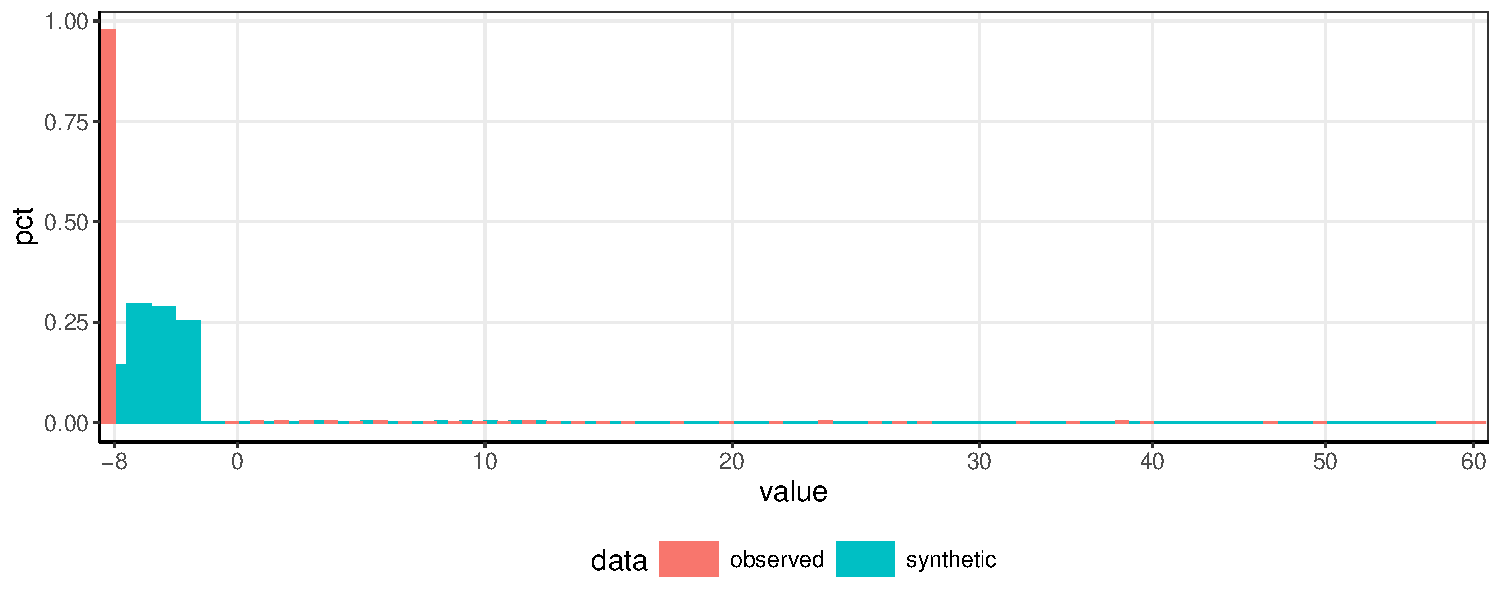
\includegraphics{../../graphs/datasynthesizer_wkabdur.pdf}}
    \label{fig:ds_variable_wkabdur}
\end{figure}
}

\frame{\frametitle{Generated variables (agegr)}
\begin{figure}
    \caption{Number of misclassified}
    \vskip -2mm
    \resizebox{\textwidth}{!}{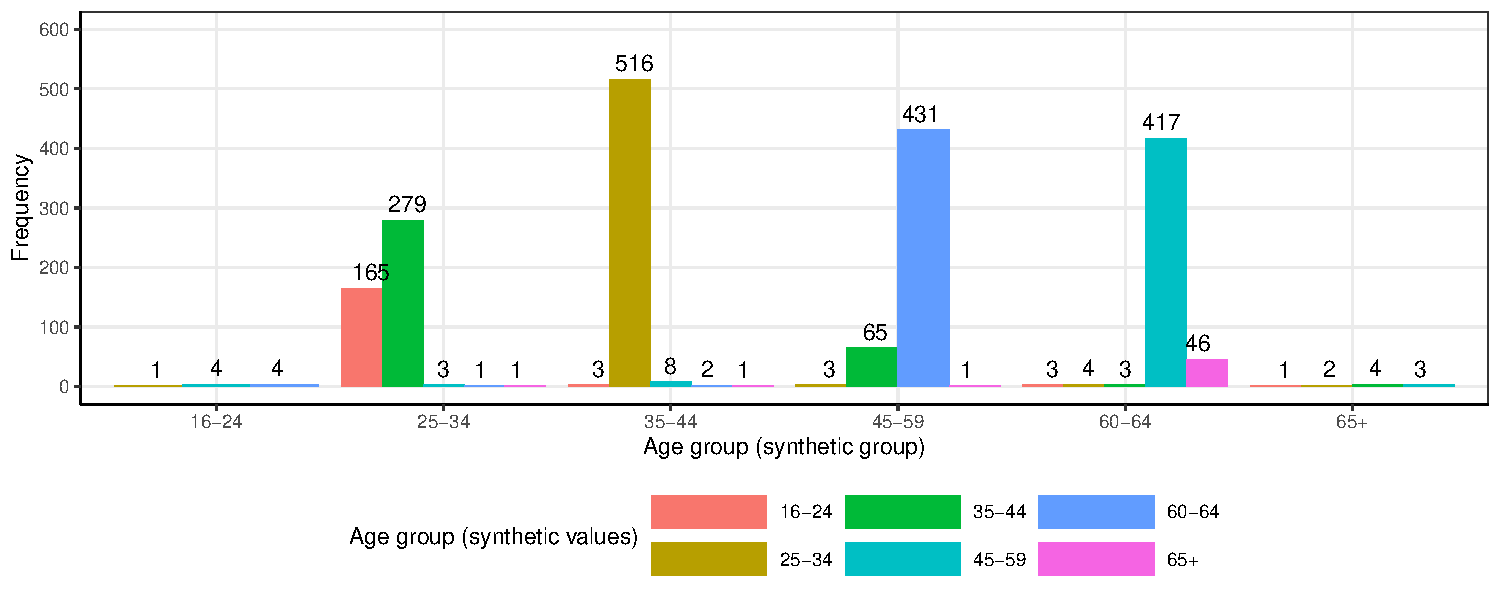
\includegraphics{../../graphs/datasynthesizer_frequency_agegr_errors.pdf}}
    \label{fig:ds_agegr_errors}
\end{figure}
}

\frame{\frametitle{Extreme values (bmi)}
\begin{figure}
    \caption{Extreme values}
    \vskip -2mm
    \resizebox{\textwidth}{!}{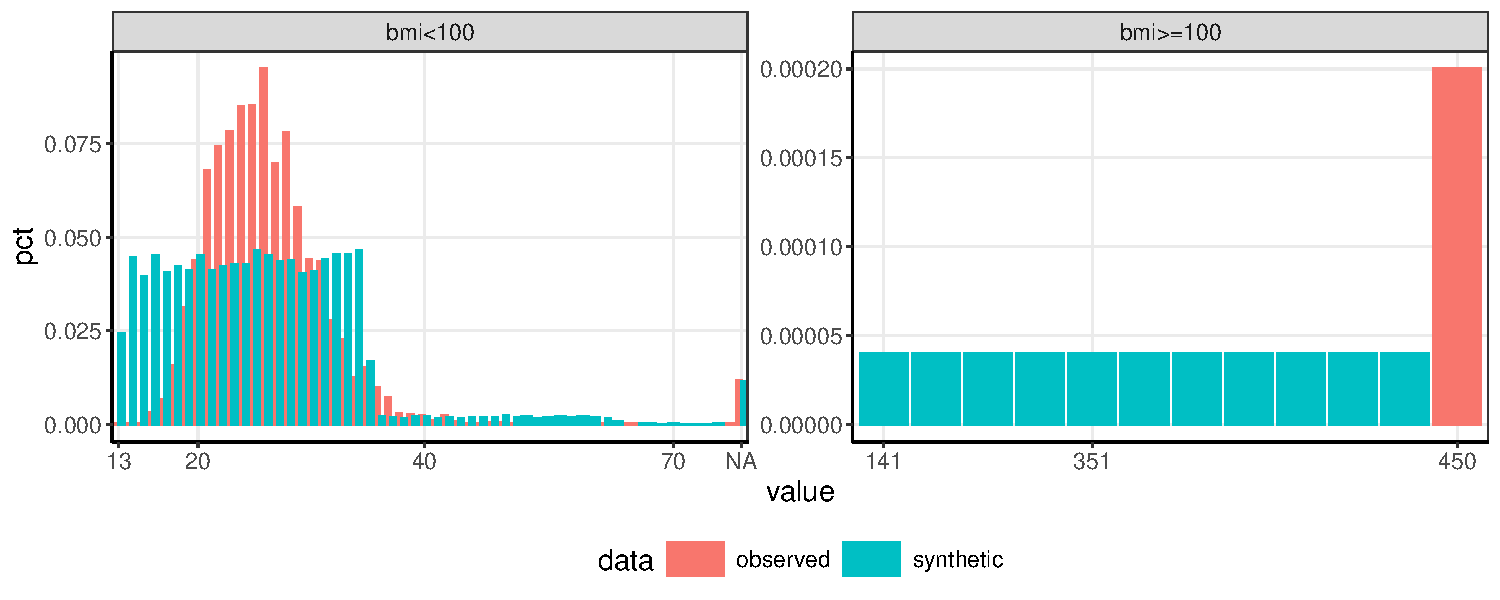
\includegraphics{../../graphs/datasynthesizer_bmi.pdf}}
    \label{fig:ds_bmi}
\end{figure}
}


\end{spacing}
\end{document}

